\chapter{Marco Introductorio}
\section{Introducci\'on}
A trav\'es de la historia, el conocimiento ha sido almacenado en gram medida de forma
escrita, teni\'endose a los libros, peri\'odicos, art\'iculos cient\'ificos, etc.,
como muestra de ello. En general este conocimiento ha sido escrito en lenguaje
natural.\\

Dada la abrumadora cantidad de este tipo de informaci\'on, surge la necesidad de su
organizaci\'on para su correcta identificaci\'on entre las diferentes \'areas de
conocimiento a las que puede pertenecer a fin de facilitar su consuta e indexaci\'on;
para este cometido es necesario contar con criterios de clasificaci\'on que faciliten
su posterior consulta.\\

El Procesamiento del Lenguaje Natural (PLN), es una rama de la Ling\"u\'istica
Computacional que b\'asicamente estudia la comunicaci\'on entre personas y m\'aquinas
por medio de lenguajes naturales. Entre las principales tareas de las que se ocupa,
se encuentra la \emph{extracci\'on de informaci\'on} que es utilizada para el
reconocimiento de nombres de entidades y extracci\'on de terminolog\'ia. \\

La extracci\'on de terminolog\'ia permite identificar y seleccionar \emph{palabras
clave} de un texto analizado, que representan su tema o motivo central, las cuales
son un criterio de clasificaci\'on eficiente. \\

Existen dos enfoques claramente identificados para la selecci\'on automatizada de
palabras clave: en base a aprendizaje supervisado y no supervisado, en el primero
la computadora es previamente entrenada con un conjunto de textos y palabras clave
seleccionadas por un experto ling\"uista para su posterior automatizaci\'on, mientras
que en el segundo la automatizaci\'on es totalmente independiente. \\

En este trabajo realizaremos la selecci\'on de palabras clave mediante un enfoque
no supervisado mediante el modelo \emph{TextRank} que utiliza algoritmos de
clasificaci\'on basados en grafos.

\section{Antecedentes}
\section{Planteamiento del problema}
\section{Objetivos}
\section{Justificativos}
\section{Aportes}
\section{L\'imites y alcanes}

\section{Metodolog\'ia}
\subsection{Metolog\'ia de desarrollo}
Scrum es una metodolog\'ia \'agil basado en un proceso iterativo e incremental, 
donde se realizan entregas parciales y regulares del producto final, obtenidas al
finalizar una iteraci\'on conocida como Sprint que tiene una duraci\'on entre 1 a 4
semanas, estas entregas son priorizadas por el beneficio que aportan al destinatario 
del proyecto, por ello esta especialmente indicado para proyectos donde se necesitan 
obtener resultados pronto o donde los requisitos son fluctuantes.

\subsubsection{Proceso Scrum}
El proceso Scrum sigue los siguientes pasos como se ve en la Figura 
\ref{fig:procesoScrum}.
\begin{enumerate}
\item Se identifican los requerimientos del sistema, descritos comos historias de
usuario o caracter\'isticas, asignandoles una prioridad y un tiempo estimado en
horas para su ejecuci\'on; obteniendo de esta manera la Pila del Producto.
\item Se seleccionan items de la Pila del Producto y se definen las tareas para su
ejecuci\'on en el siguiente Sprint.
\item Al finalizar un Sprint se reasigna una prioridad a los items de la Pila del
Producto en base a los resultados obtenidos y se planifica el siguiente Sprint.
\end{enumerate}
\begin{figure}
	\begin{center}
		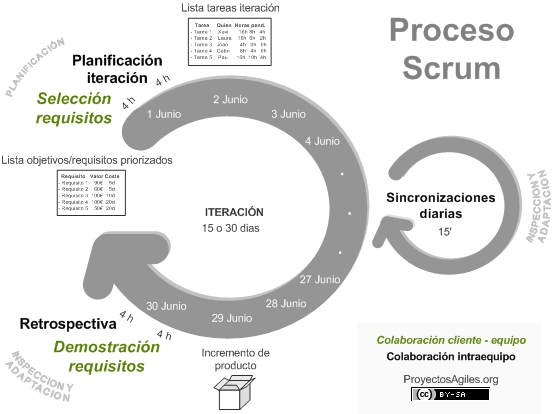
\includegraphics[scale=0.5]{./resources/img/proceso_scrum.jpg}
		\caption{\small Proceso Scrum.}
		\label{fig:procesoScrum}
	\end{center}
\end{figure}
